\documentclass[12pt]{article}

\usepackage{times}
\usepackage{textcomp}
\usepackage{listings}
\usepackage{fullpage}
\usepackage{color}
\usepackage{hyperref} 
\usepackage{pst-tree} 
\usepackage{verbatim} 
\usepackage{graphicx}
\usepackage{amsmath,amsfonts,amssymb,amsthm}
\graphicspath{ {./}} 

\def\part#1{\item[\bf #1)]}
\renewcommand{\thesubsection}{Question \arabic{subsection}}

\author{Clement Tsang}

\begin{document}

\begin{center}
\Large\textbf{CS 241, Lecture 11 - Top Down Parsing, First and Follow}
\end{center}
\begin{center}
\textbf{Thurs, Feb 14, 2019}
\end{center}

\section{Top Down Parsing}
\begin{itemize}
    \item Given a CFG $G = (N, \Sigma, P, S)$ and a terminal string $w \in \Sigma^*$, we want to find the derivation - the steps s.t. $S \Rightarrow \dots \Rightarrow w$ or prove that $w \not\in L(G)$ (just throw an error if so).
    \item Top-down parsing  says start from $S$ and try to get to $w$.
    \item Bottom-up parsing says says to start with $w$ and try to see how we could get to $w$ in the first place.
    \item We will first consider top-down parsing:
        \begin{itemize}
            \item We start with $S$ and store itermediate derivations in a stack, then match characters to $w$.  
            \item Use a stack to do so.  
            \item Every time we pop from stack, the consumed input and the reverse of the stack is equal to an intermediate step in our derivation.
            \item We augment our grammar top include $\vdash$ and $\dashv$ to symbolize the beginning and end of the file, respectively.  We also use $S'$ to indicate a new start state.
            \item We can see the algorithm described as follows: \\
                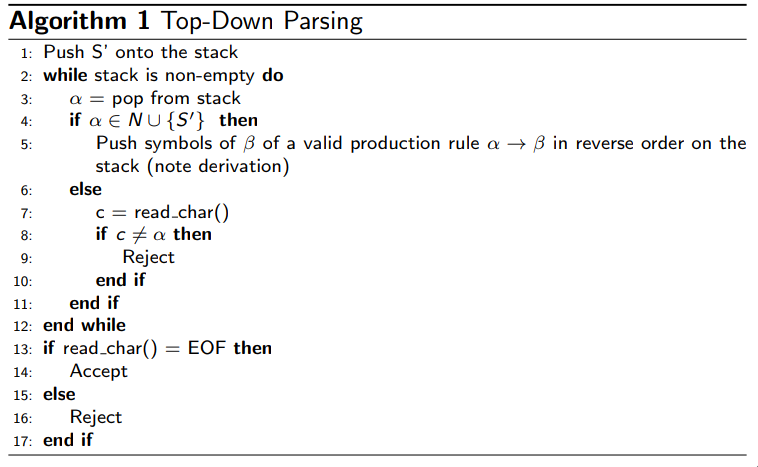
\includegraphics[scale=0.5]{top_down_alg.png}
            \item For example:
                \begin{align*}
                    S &\rightarrow AcB (1)\\
                    A &\rightarrow ab (2)\\
                    A &\rightarrow ff (3)\\
                    B &\rightarrow def (4)\\
                    B &\rightarrow ef (5)
                \end{align*}
                Determine if $w = abcdef \in L(G)$.  We add a rule:
                $$S' \rightarrow \vdash S \dashv (0)$$
                We want to look for $w = \vdash abcdef \dashv$ in this augmented grammar.  This gives us the following parse table:\\
                \begin{tabular}{c|c|c|c}
                    Stack & Read & Processing & Action\\
                    \hline
                    S' & $\epsilon$ & $\vdash$ abcdef $\dashv$ & Pop S', push $\dashv$, $\vdash$ (Rule 0) \\
                    $\dashv$ S $\vdash$ & $\epsilon$ & $\vdash$ abcdef $\dashv$ & Match $\vdash$ \\
                    $\dashv$ S & $\vdash$ & abcdef $\dashv$ & Pop S, push B, c, A (Rule 1) \\
                    $\dashv$ BcA & $\vdash$ & abcdef $\dashv$ & Pop A, push b, a (Rule 2) \\ 
                    $\dashv$ Bcba & $\vdash$ & abcdef $\dashv$ & Match a \\
                    $\dashv$ Bcb & $\vdash$ a & bcdef $\dashv$ & Match b \\
                    $\dashv$ Bc & $\vdash$ ab & cdef $\dashv$ & Match c \\
                    $\dashv$ B & $\vdash$ abc & def $\dashv$ & Pop B, push f, e, d (Rule 4) \\
                    $\dashv$ fed & $\vdash$ abc & def $\dashv$ & Match d \\
                    $\dashv$ fe & $\vdash$ abcd & ef $\dashv$ & Match e \\
                    $\dashv$ f & $\vdash$ abcde & f $\dashv$ & Match f \\
                    $\dashv$ & $\vdash$ abcdef & $\dashv$ & Match $\dashv$ \\
                    $\epsilon$ & $\vdash$ abcdef $\dashv$ & $\epsilon$ & Accept, as stack = input = $\epsilon$
                \end{tabular}
            \item When we popped $A$, we had multiple possible choices - which rule would we use?
            \item We construct a predictor table, using a single character that we look at, to tell us which rule to use.  For our example, for $A$, if we see an $a$, then we use rule 2; if we see a $f$ then use rule 3.
            \item But this won't work if we have an element that contains more than one other element - for example, if we add a new rule $A \rightarrow adf$.
        \end{itemize}
\end{itemize}
\newpage

\section{First and Follow}
\begin{itemize}
    \item A $LL(1)$ grammar is one that each cell of the predictor tables contains at most \textbf{one} entry.
    \item With an $LL(1)$ grammar, we can drop the set notation from the predictor table.
    \item We call it $LL(1)$ as:
        \begin{itemize}
            \item First L: Scan left to right
            \item Second L: Leftmost derivations
            \item Number of symbols in lookahead: 1
        \end{itemize}
    \item Constructing the lookahead table - we define four functions:
        \begin{itemize}
            \item \emph{Nullable}$(\beta) = $true iff $\beta \Rightarrow^* \epsilon$ and false otherwise
            \item \emph{Follow}$(A) = \{b \in \Sigma' : S' \Rightarrow^* \alpha Ab \beta$ for some $\alpha, \beta \in V^*\}$
            \item \emph{Predict}$(A, a) = \{A \rightarrow \beta : a \in $ \emph{First}$(\beta)$\}
            \item \emph{First}$(\beta) = \{a \in \Sigma` : \beta \Rightarrow^* a\gamma$, for some $\gamma \in V^*\}$
        \end{itemize}
    \item More informally:
        \begin{itemize}
            \item \emph{Nullable($\beta$)}: boolean function, for $\beta \in V^*$ is true iff $\beta \Rightarrow^* \epsilon$.
            \item \emph{Follow(A)}: for any $A \in N'$, this is the set of elements of $\Sigma'$ that can come immediately after $A$ in a derivation starting from $S'$.
            \item \emph{Predict(A, a)}: production rules that apply when $A \in N'$ is on the stack, and $a \in \Sigma'$ is the next input character.
            \item \emph{First($\beta$)}: set of characters that can be the first letter of a derivation starting from $\beta \in V^*$.
        \end{itemize}
    \item Note our definition of \emph{Predict} is not correct right now.
    \item Our predict table looks like this: \\
        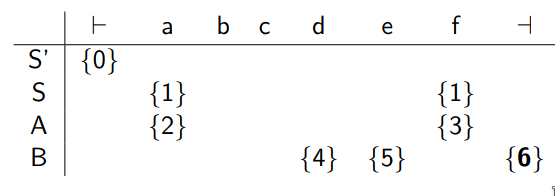
\includegraphics[scale=0.5]{aug_predict.png}
    \item We can see \emph{First} with our previous example:\\
        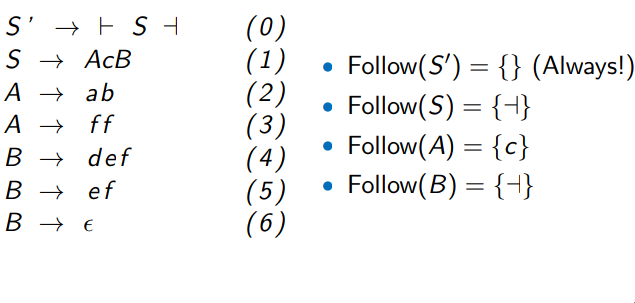
\includegraphics[scale=0.5]{first_example.png}
    \item We say that a $\beta \in V^*$ is \textbf{nullable} iff \emph{Nullable}($\beta$) = true
    \item Redefine \emph{Predict}$(A, a) =  \{A \rightarrow \beta : a \in$ \emph{First}$(\beta)\} \cup \{A \rightarrow \beta : \beta$ is nullable and $a \in$ \emph{Follow(A)}\}
    \item Note this ALL only works well for $LL(1)$. We will make our grammar work with $LL(1)$, and thus, these rules!
\end{itemize}

\end{document}
